Analiza la figura geométrica obten la expresión algebraica para el \textbf{perímetro} de las siguientes figuras:

\begin{multicols}{2}
    \begin{parts}
        {\printanswers
            \centering 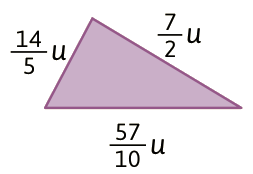
\includegraphics[width=0.2\textwidth]{../images/20230319021512}
            \begin{solutionbox}{2cm} $P=\left(\frac{14}{5} \text{ u}\right)+\left(\frac{7}{2}\text{ u}\right)+\left(\frac{57}{10}\text{ u}\right)=\frac{120}{10}\text{ u}=12 \text{ u} $\end{solutionbox}
        }
        \centering 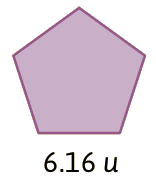
\includegraphics[width=0.11\textwidth]{../images/20230319021457}
        \begin{solutionbox}{1.5cm}\[P=5 \left( 6.16 \text{ u}\right)=30.8\]\end{solutionbox}


        \centering 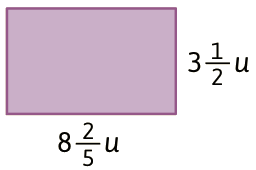
\includegraphics[width=0.2\textwidth]{../images/20230319021443}
        \begin{solutionbox}{2cm}$P=2 \left( 3\dfrac{1}{2} \text{ u}\right)+2 \left( 8\dfrac{2}{5} \text{ u}\right)=23\dfrac{4}{5} \text{ u}$\end{solutionbox}

        \centering 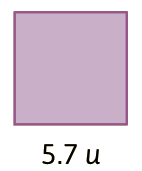
\includegraphics[width=0.1\textwidth]{../images/20230319021432}
        \begin{solutionbox}{1.5cm}$P=4 \left( 5.7 \text{ u}\right)=22.8 \text{ u}$\end{solutionbox}

        \centering 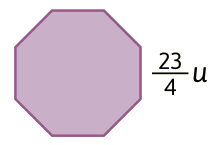
\includegraphics[width=0.16\textwidth]{../images/20230319021504}
        \begin{solutionbox}{2cm}$P=8 \left( \dfrac{23}{4} \text{ u}\right)=46\text{ u}$\end{solutionbox}

        \centering 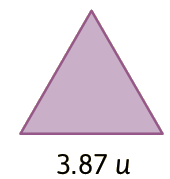
\includegraphics[width=0.12\textwidth]{../images/20230319021450}
        \begin{solutionbox}{1.5cm}$P=3 \left( 3.87 \text{ u}\right)=11.61\text{ u}$\end{solutionbox}
    \end{parts}
\end{multicols}
